
\chapter{An Analytical Pulse Approximation Algorithm for Multiple Event Transients} \label{ch2}

As the transistor size has continued to decrease, the probability of a SEU occurring has continued to greatly increase. This, in effect, has created a need for accurate and efficient SEU simulators. The SEU problem has been investigated deeply. \cite{MARS_C,SERA,FASER} However, due to the close proximity of transistors and the increase in transistor error sensitivity, the probability of a single or multiple radiation strikes producing multiple voltage pulses has become a concern. The authors in \cite{Harada} investigated a 65 nm 3x3 inverter matrix and found that 40\% of all single radiation strikes resulted in the generation multiple significant voltage pulses. Considering the possibility that a modern circuit is also vulnerable to multiple simultaneous strike, there is a significant concern for multiple transients. This creates the need for either the enhancement of existing SEU tools or the development of new tools which can consider the single event multiple transient (SEMT) and multiple event multiple transient (MEMT) effect.

Previous work in SEU’s have shown that combinational circuits are vulnerable to 3 types of error masking effects: logical masking, electrical masking and temporal masking. Accurate estimation of the soft error rate requires consideration of all masking factors for not only SEU’s but also the SEMT and MEMT cases. In this paper, the focus is on the consideration of the electrical masking effect. There have been many approaches to the electrical masking problem for the SEU case \cite{Omana_Trap,Accurate_Masking,Weibull}. However, a major drawback with these approaches is that they do not accurately consider the effect of multiple pulses occurring on the gate input (referred to as convergent pulses). Since, in the SEMT and MEMT cases, there are many pulses generated, the occurrence of convergent pulses is much higher. To model these cases, an accurate electrical masking model must consider convergent pulses. 

There has been a few attempts at modeling the effect multiple transient pules, however all approaches suffer from inaccurate estimation of electrical masking. The authors in \cite{METSys,TahooriMET} both proposed a simulation tool to determine the soft error rate (SER) of a combinational circuit in the presence of multiple transients, however, they calculate the output transient of a gate with a convergent input through the simple superposition of the pulse widths. As stated in \cite{Accurate_Masking}, this is insufficient since accurate electrical masking modeling requires the inclusion of the pulse amplitude and non-linear portions of the glitch.

An additional possible solution to the pulse convergence problem is the simple extension of \cite{Accurate_Masking} for convergent pulses. In \cite{Accurate_Masking} an accurate iterative model for the single pulse case is proposed. Their model can easily be extended by generating larger look-up tables. However, since they characterize stacked transistors using look-up tables, gates with more than 2-inputs require tables with 125,000 entries for 3-input gates and over 7 million for 4-input gates. Thus our model provides an enhancement to \cite{Accurate_Masking} by allowing the characterization of stacked transistors using a look-up tables for the transistor and the Miller capacitance between the gate and drain terminals.

Based on the above discussion, there is a lack of accurate and fast methods to consider convergent pulses.  This provides the motivation of this work. To the author’s knowledge, the proposed model is the first masking model that accurately and efficiently approximates the entire output pulse shape for convergent input pulses. Through extensive experimentation, the proposed model has been shown to be robust for various input shapes and process technologies while providing a 15X speed-up over HSPICE.

\section{Pulse Approximation Model}
As in \cite{Accurate_Masking}, an important aspect of the proposed model is the accurate approximation of the transistor drain to source current (IDS). To consider the $I_{DS}$ current, a look-up table for each transistor is created by sweeping both the gate-source voltage (VGS) and the drain-source voltage ($V_{DS}$).
 
Additionally, as in \cite{Accurate_Masking}, the effects of pulse overshoot and undershoot are considered through the use of a Miller capacitor. In contrast to \cite{Accurate_Masking}, however, we consider the MOS parasitic effects on each individual transistor through the inclusion of a Miller capacitance between the gate and drain terminals. While in practice there may be a capacitance between the gate and source, it was found through numerous simulations that this effect was negligible Fig. \ref{TModel} demonstrates the proposed model for a NMOS and a PMOS transistor. 

\begin{figure}[!htbp]
	\centering
	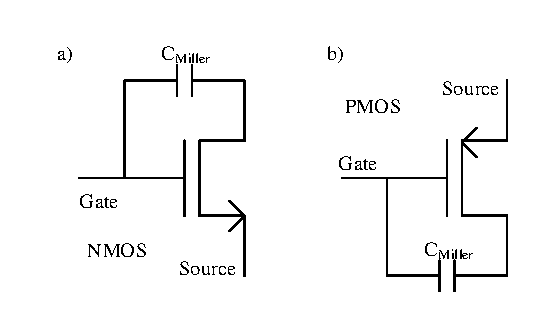
\includegraphics[width=0.50\linewidth]{Figures/TransistorModel}
	%where an .eps filename suffix will be assumed under latex, 
	%and a .pdf suffix will be assumed for pdflatex; or what has been declared
	%via \DeclareGraphicsExtensions.
	\caption{(a) The transistor model used for a NMOS. (b) The transistor model for a PMOS.}
	\label{TModel}
\end{figure}

As stated in \cite{Accurate_Masking}, it was observed that the value of the Miller capacitance varied over the range of drain-source ($V_{DS}$) and gate-source ($V_{GS}$) voltages. To consider this effect, it is proposed to generate a look-up table with each entry pertaining to the Miller capacitance at each specific $V_{GS}$ and $V_{GS}$ bias. The Miller capacitance look-up tables can be characterized using HSPICE by sweeping the $V_{GS}$ and $V_{GS}$ voltages and measuring the current flowing through the gate node of the transistor ($i_m$). Using the current $i_m$, the derivative of the difference between the gate and drain voltages and equation \ref{Millereq}, the capacitance $C_{Miller}$ can be calculated.

\begin{equation}\label{Millereq}
C_{Miller} = \frac{i_m}{\frac{d(V_{DS}-V_{GS})}{dt}}
\end{equation}

As stated before, the IDS current and the Miller capacitance for both the PMOS and NMOS transistors are characterized. Using this data, each transistor is modeled as a current source and its Miller capacitor. Any given gate can then be represented by replacing each transistor with a current source and a Miller capacitor connected between the drain and gate terminals. At the output of the gate, a load capacitance is added to consider the gate loading effects and to calibrate the model. Fig. \ref{Convert} demonstrates the conversion to the proposed model on a 2-input NAND gate.

\begin{figure}[!htbp]
	\centering
	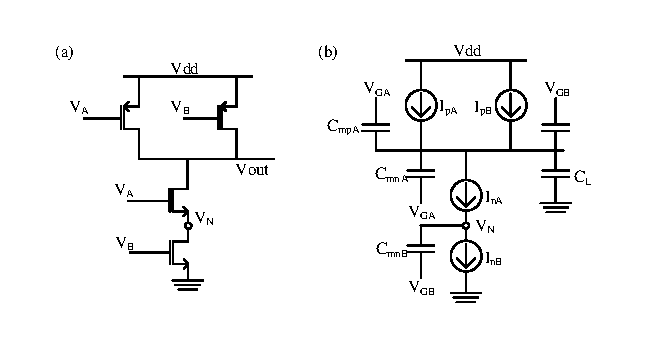
\includegraphics[width=0.85\linewidth]{Figures/Conv_Mod}
	%where an .eps filename suffix will be assumed under latex, 
	%and a .pdf suffix will be assumed for pdflatex; or what has been declared
	%via \DeclareGraphicsExtensions.
	\caption{(a) The transistor model used for a NMOS. (b) The transistor model for a PMOS.}
	\label{Convert}
\end{figure}

Before beginning the discussion on the equation derivation it is important to note that this model is general for all types of gates but for the sake of this discussion, the derivation will focus on CMOS NAND and NOR gates.  

The proposed gate modeling for a given gate, as in Fig \ref{Convert}b, can be generalized for an $i$ number of inputs as in Fig. \ref{Gmod} where a single current source represents the current for the pull-up network and a second current source represents the pull-down network. This is based on the assumption that the gate is a CMOS gate in which one network consists of parallel current sources and the equivalent current is equal to the sum of each parallel transistor current. The other current source represents the current flowing through series connected transistors which ideally have a single constant current. However, in practice, due to parasitic effects, the current in each stacked transistor varies. It was found through many simulations that the best approximation for this current was by taking the average between each transistor current in the stack. For example, if we have the circuit in Fig. \ref{Convert}b, the current on the stacked transistors can be calculated using the following equation:

\begin{equation}\label{pdeq}
I_{pd} = \frac{I_{nA}+I_{nB}}{2}
\end{equation}

\begin{figure}[!htbp]
	\centering
	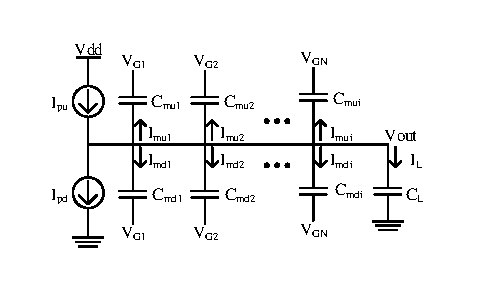
\includegraphics[width=0.75\linewidth]{Figures/GenModel}
	%where an .eps filename suffix will be assumed under latex, 
	%and a .pdf suffix will be assumed for pdflatex; or what has been declared
	%via \DeclareGraphicsExtensions.
	\caption{A generalized representation of the gate model.}
	\label{Gmod}
\end{figure}

To derive the output equation for the node $V_{out}$ in Fig. \ref{Gmod}, we first use Kirchoff’s Current Law (KCL) at the node $V_{out}$. Assuming that $I_{mu_i}$ and $I_{md_i}$ are the currents through the $i$-th Miller capacitor, $I_L$ is the current through the load capacitor and $I_{pu}$ and $I_{pd}$ represent the pull-up and pull-down current respectively, KCL will result in the following:

\begin{equation}\label{KCL}
I_{pu} = I_{pd} + I_L + \sum_{i=1}^{N}I_{mu_i} + \sum_{i=1}^{N}I_{md_i}
\end{equation}

For our model, we discretized the time into time steps with the variable $t_step$. Additionally, we represent each variable in the current time instant with the subscript $i$ and each variable in the previous time instant with the subscript $i-1$. Lastly, we represent the change in a value between two time instances using $\Delta$ (i.e. $V_i-V_{i-1}=\Delta V$). 

According to the charge conservation law, we get equation \ref{miller} for each Miller capacitor $C_{m_i}$ connected between $V_{out}$ and the input voltage $V_{G_i}$.

\begin{equation}\label{miller}
I_{m_i} = \frac{[\Delta V_{out} - \Delta V_{G_i}]C_{m_i}}{t_{step}}
\end{equation}

Next, consideration of the load capacitance $C_L$ gives the following equation:

\begin{equation} \label{load}
I_L = \frac{(\Delta V_{out}C_L)}{t_{step}}
\end{equation}

By substituting into equation \ref{KCL} the current $I_{m_i}$ from \ref{miller} for the currents $I_{mu_i}$ and $I_{md_i}$ and replacing the current $I_L$ with equation \ref{load}, we get the following for a $N_u$ number of Miller capacitors connected between $V_{out}$ and the $i$-th input in the pull-up network (denoted by $C_{mu_i}$ and a $N_d$ number of Miller capacitors connected to $V_{out}$ and the $i$-th input on the pull-down network (denoted by $C_{md_i}$): 

\begin{equation} \label{md1}
I_{pu} = I_{pd} + \frac{(\Delta V_{out}C_L)}{t_{step}} + \sum_{i=1}^{N_u} \frac{[\Delta V_{out} - \Delta V_{G_i}]C_{mu_i}}{t_{step}} + \sum_{i=1}^{N_d} \frac{[\Delta V_{out} - \Delta V_{G_i}]C_{md_i}}{t_{step}}
\end{equation} 

Rearranging \ref{md1} and solving for $\Delta V_{out}$ gives the following:

\begin{equation} \label{md2}
\Delta V_{out} = \frac{(I_{pu}-I_{pd})t_{step} + \sum_{i-1}^{N_u} \Delta V_{G_i}C_{mu_i} + \sum_{i=1}^{N_d} \Delta V_{G_i}C_{md_i}}{C_L + \sum_{i=1}^{N_u}C_{mu_i} + \sum_{i=1}^{N_d}C_{md_i}}
\end{equation}

Assuming that $\Delta V_{out_i}$ equals $V_{out_i} - V_{out_{(i-1)}}$ results in:

\begin{equation} \label{mdf}
V_{out_i} = \Delta V_{out} + V_{out_{i-1}}
\end{equation}

As can be observed in equations \ref{md2} and \ref{mdf} an important aspect of the proposed model is the accurate consideration of both the pull-up and pull-down currents. As stated before, cases where the pull-up or pull-down transistors are composed of parallel connected transistors the current can simply be found through the sum of the drain to source currents. However, in cases where the transistors are in series, the determination of the equivalent current is more complicated.

In Fig. \ref{Convert}a the pull-down branch consists of series connected NMOS transistors which will be used to demonstrate the derivation. Note that using the same method, the equations for stacked PMOS devices can be easily derived. Within the stack there is an intermediate node voltage $V_n$ which is crucial for the determination of the drain to source currents in the transistors. Through many simulations using the transistor drain to source current look-up tables, it was found that accurate approximation of the node voltages provided accurate current values for each transistor in the stack. 

To calculate the intermediate voltage, it is proposed to first convert each transistor to the representations in Fig. \ref{TModel}a and \ref{TModel}b. which results in the circuit in Fig. \ref{Convert}b. In Fig. \ref{Convert}b. the intermediate node voltage $V_n$ is connected to a static capacitor representing the loading effect of the subsequent transistor stack. Next, the node voltage equation will be derived.

Similar to equation \ref{md2}, the node voltage $V_n$ is modeled using discrete time steps. Using KCL at $V_n$ in Fig. \ref{Convert}b we get the following equation:

\begin{equation} \label{KCLNode}
I_{D1} = I_{D2} + I_m
\end{equation}

As in equation \ref{miller}, the current through the static capacitor can be determined using the charge conservation law resulting in the following for the current $I_m$.

\begin{equation} \label{millernode}
I_m = \frac{C_{m1}(V_{n_i} - V_{n_{i-1}})}{t_{step}}
\end{equation}

By substituting \ref{millernode} into \ref{KCLNode} and solving for $V_{n_i}$, the equation for the node voltage $V_n$ at the time instant $i$ is derived.

\begin{equation} \label{nvolt}
V_{n_i} = \frac{(I_{D1} - I_{D2})t_{step}}{C_{m1}} + V_{n_{i-1}}
\end{equation}

In cases where there are more than 2 stacked transistors, the described model is directly extendable for each intermediate node. Fig. \ref{StackT}a and b provides the conversion for 3 stacked NMOS transistors to our model. The node voltages $V_{N1}$ and $V_{N2}$ can be found in any order using equation \ref{nvolt} and by considering the currents flowing into the node. For example, to solve for the node voltage $V_{N2}$ the currents $I_{D2}$ and $I_{D3}$ would be used in equation \ref{nvolt} since they are directly connected to the node. Additionally, the order for solving the node equations does not matter since the node voltages from the previous step $i-1$ are used.

\begin{figure}[!htbp]
	\centering
	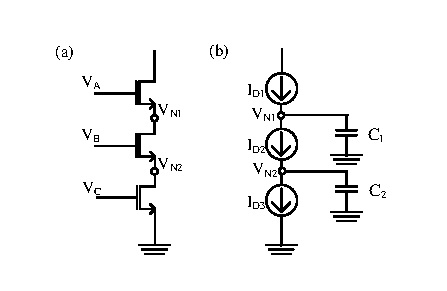
\includegraphics[width=0.70\linewidth]{Figures/Stacked}
	%where an .eps filename suffix will be assumed under latex, 
	%and a .pdf suffix will be assumed for pdflatex; or what has been declared
	%via \DeclareGraphicsExtensions.
	\caption{(a) Three stacked NMOS transistors with two intermediate nodes $V_{N1}$ and $V_{N2}$. (b) The transistors converted to the proposed circuit model.}
	\label{StackT}
\end{figure}

\section{Experimental Results}

The proposed algorithm was implemented in Matlab and characterized using the 32 nm and 45 nm PTM library \cite{PTM} and the 65 nm IBM library. To test the proposed model, three benchmark circuits for each process library were created to test two convergent pulses on a 2 and 3 input NAND gate and a 2 input NOR gate. The first two benchmark circuits denoted by NAND2R and NAND2F in column 1 of Table \ref{table:pt}, consists of two NAND gate chains with each off-input held to a non-controlling value. The chains contain two gates and the R and F in the benchmark names represent either a rising (R) or falling (F) pulse on the convergent gate’s inputs. Each chain is then connected to an input of the NAND gate. The benchmark circuits NOR2R and NOR2F are constructed similarly but the chains consist of NOR gates and are connected to the input of a 2-input NOR gate. The last benchmark circuits constructed, NAND3R and NAND3F, were created with two, 2-gate chains connected to the first and second input of the 3-input NAND gate. The remaining off-input was held to a non-controlling value. 

Next, to accurately model the injected pulse shape, the injection current is represented as a current source located at the output of the first gate in the chain. We then used the function for the pulse shape given in \cite{injeq} to relate the strike current to a given charge. Equation \ref{qeq} was used to model the current generated by a pulse strike.

Using equation \ref{qeq}, $Q_o$ was varied over a range of charge values that results in an observable error. For our test cases, we found that a charge ranging from 3-16 fC for a τ of $90x10^{-12}$ provided an observable output shape for all processes tested. We then propagated the pulses through the gate chains to gate of interest and compared the generated outputs using the proposed model and the model in \cite{Accurate_Masking} to HSPICE. Table \ref{table:pt} details the average error for 30 cases per gate and transition type for the 32, 45 and 65 nm processes using 2400 data points over a range of 0 to 1.2 pico-seconds. While the variable $t_{step}$ could adaptively change with the pulse shape, $t_{step}$ was set to a fixed value since simulation time was minimized by limiting the number of points to the expected maximum pulse width. This ensured that the vector storing the pulse shape contained the pulse information and did not have extra unnecessary values. The first column gives the benchmark name. All subsequent columns provide the MSE error for each test case for the proposed method and the method in \cite{Accurate_Masking}. Assuming that $N$ represents the number of calculated points, $V_i^H$ represents the pulse voltage at point $i$ on the signal from HSPICE and $V_i^C$ is the voltage calculated by the proposed model, the MSE was calculated using the following equation:

\begin{equation}
MSE = \frac{\sum_{i=0}^{N} (V_i^H - V_i^C)^2}{N}
\end{equation}

As can be seen from Table \ref{table:pt}, the proposed model is much more accurate over the model proposed in \cite{Accurate_Masking}. In all tested cases, the method in \cite{Accurate_Masking} predicted there would be an output pulse. However, they only propagate the pulse with the largest width which fails to consider the effect of multiple pulses and provides a pulse with a much smaller width. For this reason, their method tends to underestimate the severity of the pulse in the presence of convergent pulses. According to Table \ref{table:pt}, our method closely predicts the output pulse shape.

Next, we run a simulation to observe how the number of points selected relates to the speed and accuracy. In this simulation, we used the NAND2F and NAND3F benchmark and applied a pulse to each input of the terminating NAND gate. We then varied the number of output data points for the terminating NAND gate in both HSPICE and the proposed model. Table \ref{table:extime} provides the results of this simulation.

The first column provides the number of simulation points used to calculate the result. Columns 2 and 3 provide the error of the proposed model and \cite{Accurate_Masking} for the given number of points. Columns 4, 5 and 6 gives the execution time of the proposed method, the method in \cite{Accurate_Masking} and HSPICE respectively. As can be seen from Table \ref{table:extime}, the reduction in simulation time scales linearly to the reduction in simulation points. 

In Fig. 5, we provide the output waveform of the simulation in Table 2 for 900 and 300 points respectively. As can be observed in Fig. 5a, the result for the proposed model closely matches the result obtained in HSPICE when 900 simulation points are used. If a higher accuracy is desired, the proposed model provides a near perfect match with 2400 points. For both the 900 and 300 point cases, it can be observed that the method in \cite{Accurate_Masking} greatly underestimates the resulting pulse thus providing a high MSE. The proposed model provides an accurate result with an MSE of 7.40x10-3 while still providing a speed-up of 15X compared to HSPICE for this benchmark. In general we have observed a speed-up of 15X for any 2-input gate using 900 points while maintaining a high accuracy.
  
In Fig. 6a and 6b, we provide the output waveforms for the NAND3F simulation for 900 and 300 points respectively. Similar to the NAND2F benchmark, a simulation with 900 points provides a close waveform approximation. However, if a lower accuracy is tolerable, the number of points can be reduced further providing a faster simulation time as demonstrated in Table \ref{table:extime} and Fig. 6b. As can be observed in Table 2, proposed model provides a speed-up of 12X for the 900 point case. In general for any 3-input gate, we have observed a speed-up of 12X using 900 points while maintaining a high accuracy

\begin{table}[!htbp]
	\begin{center}
		\caption{Proposed and \cite{Accurate_Masking} compared to HSPICE for 2400 points.}
		\label{table:pt}
		\begin{tabular}{|c|c|c|c|c|c|c|}
			\hline
			Circuit & \multicolumn{2}{c|}{MSE [65nm] ($x10^{-3}$)} & \multicolumn{2}{c|}{MSE [45nm] ($x10^{-3}$)} & \multicolumn{2}{c|}{MSE [32nm] ($x10^{-3}$)} \\ 
			\cline{2-7}
			& Proposed & \cite{Accurate_Masking} & Proposed & \cite{Accurate_Masking} & Proposed & \cite{Accurate_Masking}\\
			\hline
			NAND2R & 0.760 & 108 & 0.453 & 35.6 & 0.190 & 45.6 \\
			\hline
			NAND2F & 1.000 & 110 & 0.550 & 67.8 & 0.467 & 50.9 \\
			\hline
			NOR2R & 0.220 & 23.0 & 0.345 & 133.0 & 0.405 &146.0 \\
			\hline
			NOR2F & 0.986 & 103 & 0.678 & 42.5 & 0.493 & 33.9 \\
			\hline
			NAND3R & 0.887 & 115 & 0.785 & 55.6 & 0.352 & 39.2 \\
			\hline
			NAND3F & 0.998 & 98.9 & 0.467 & 39.8 & 0.465 & 30.8 \\
			\hline
		\end{tabular}
	\end{center}
\end{table}

\begin{table}[!htbp]
	\begin{center}
			\caption{Execution Time vs Accuracy ($x10^{-3}$)}
			\label{table:extime}
			\begin{tabular}{|m{5em}|m{5em}|m{5em}|m{5em}|m{5em}|m{5em}|}
				\hline
				Points & Error \newline Proposed & Error \cite{Accurate_Masking} & Execution Time Proposed & Execution Time \cite{Accurate_Masking} & Execution Time HSPICE \\
				\hline
				\multicolumn{6}{|c|}{NAND2F} \\
				\hline
				2400 & 0.486 & 85.7 & 8.39 & 8.03 & 100\\
				\hline
				1200 & 3.90 & 92.0 & 4.34 & 4.01 & 60 \\
				\hline
				900 & 7.40 & 97.8 & 3.43 & 3.05 & 50 \\
				\hline
				300 & 41.1 & 115.9 & 1.23 & 1.18 & 20 \\
				\hline
				\multicolumn{6}{|c|}{NAND3F} \\
				\hline
				2400 & 0.529 & 37.5 & 12.1 & 11.4 & 120\\
				\hline
				1200 & 6.40 & 38.7 & 6.40 & 5.90 & 70 \\
				\hline
				900 & 13.0 & 42.8 & 4.90 & 4.50 & 60 \\
				\hline
				300 & 60.9 & 85.0 & 1.91 & 1.50 & 30 \\
				\hline
			\end{tabular}
	\end{center}
\end{table}

\begin{figure}[!htbp]
	\[\begin{gathered}
	\hbox {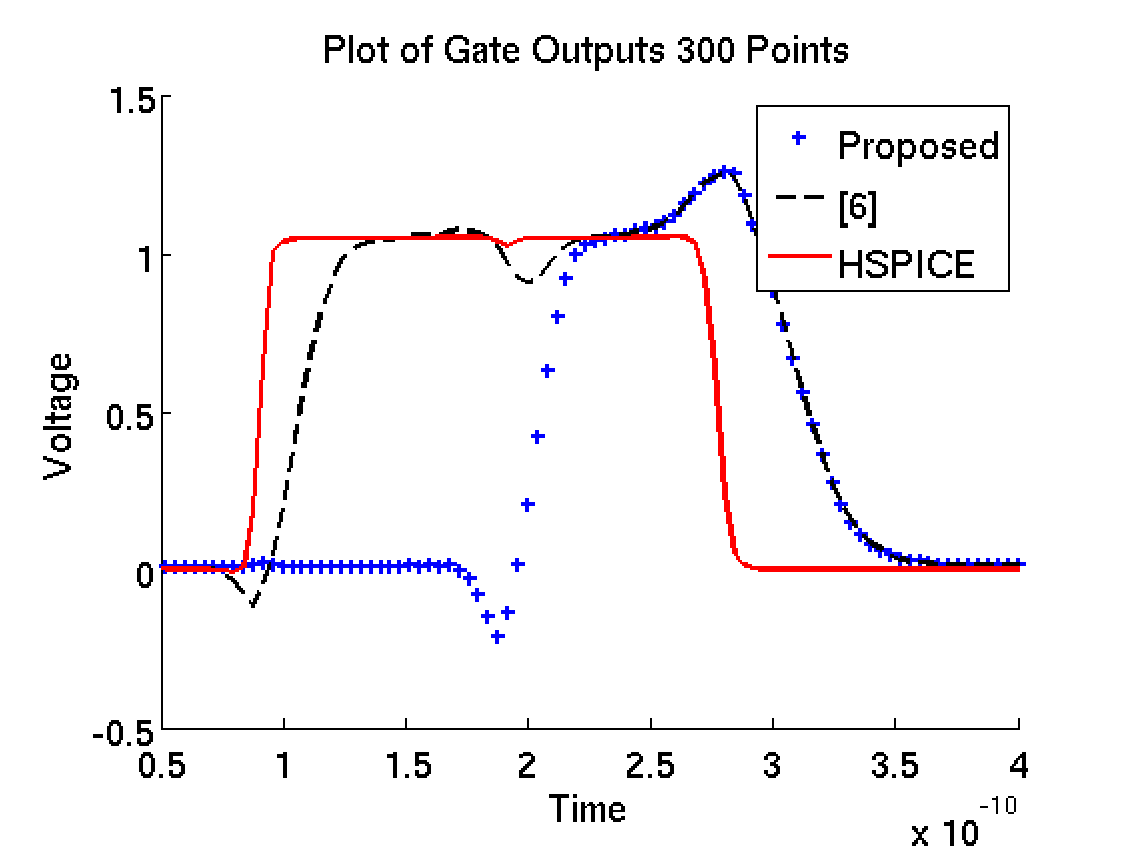
\includegraphics[width=0.45\linewidth]{Figures/plot300}}
	\quad
	\hbox {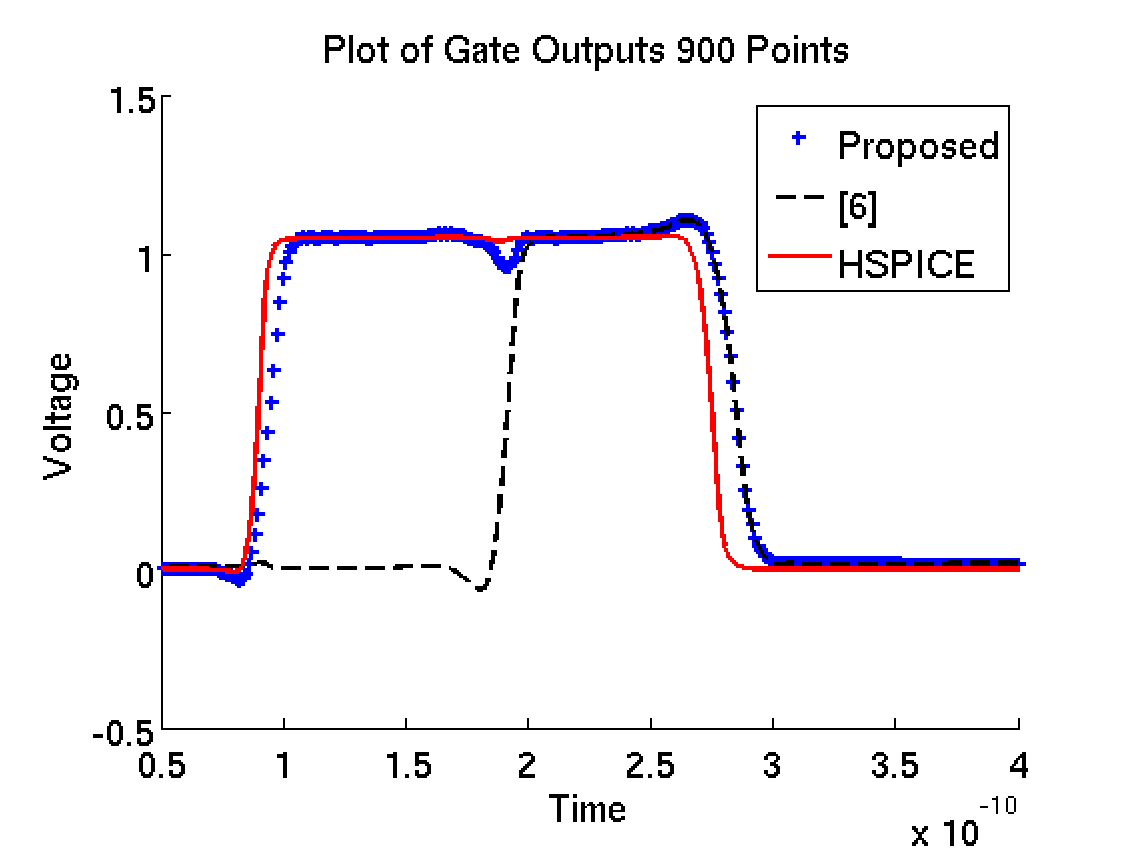
\includegraphics[width=0.45\linewidth]{Figures/plot960}} \\
	\hbox to 3in{\hfill(a)\hfill} \quad \hbox to 3in{\hfill(b)\hfill}
	\end{gathered}\]	
	\caption{(a) Output of NAND2F with 300 points. \ (b) Output of NAND2F with 900 points}
	\label{NAND2_pt}
\end{figure}

\begin{figure}[!htbp]
	\[\begin{gathered}
	\hbox {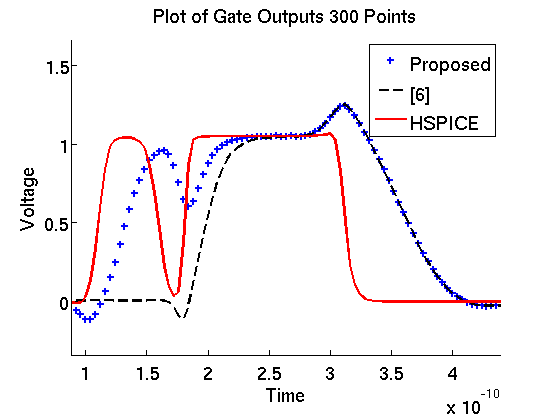
\includegraphics[width=0.45\linewidth]{Figures/plotoutnand3300}}
	\quad
	\hbox {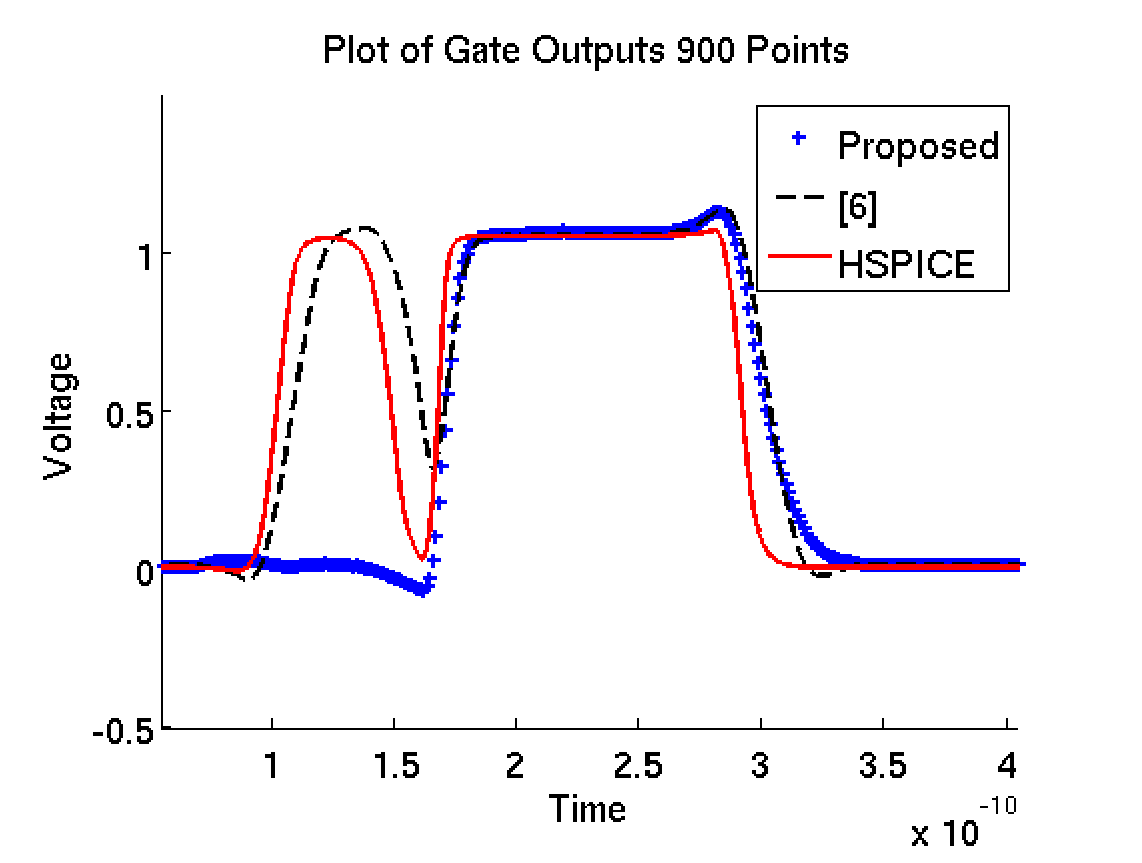
\includegraphics[width=0.45\linewidth]{Figures/plotoutnand3903}} \\
	\hbox to 3in{\hfill(a)\hfill} \quad \hbox to 3in{\hfill(b)\hfill}
	\end{gathered}\]	
	\caption{(a) Output of NAND3F with 300 points. \ (b) Output of NAND3F with 900 points}
	\label{NAND3_pt}
\end{figure}

\section{Conclusion}
In this section, a model was proposed that improves SEMT and MEMT error simulation by calculating the output pulse shape in the presence of convergence with an MSE of less than $7.40x10^{-3}$ for 2-input gates and 13x10-3 for 3-input gates  using 900 points and a speed-up of 15X and 12X respectively compared to HSPICE. Future work with our model includes the study of the number of points effect the simulation result on large benchmarks and the study of SEMT and MEMT on large standard benchmark circuits using the proposed model. 